% Options for packages loaded elsewhere
\PassOptionsToPackage{unicode}{hyperref}
\PassOptionsToPackage{hyphens}{url}
%
\documentclass[
  11pt,
  ignorenonframetext,
]{beamer}
\usepackage{pgfpages}
\setbeamertemplate{caption}[numbered]
\setbeamertemplate{caption label separator}{: }
\setbeamercolor{caption name}{fg=normal text.fg}
\beamertemplatenavigationsymbolsempty
% Prevent slide breaks in the middle of a paragraph
\widowpenalties 1 10000
\raggedbottom
\setbeamertemplate{part page}{
  \centering
  \begin{beamercolorbox}[sep=16pt,center]{part title}
    \usebeamerfont{part title}\insertpart\par
  \end{beamercolorbox}
}
\setbeamertemplate{section page}{
  \centering
  \begin{beamercolorbox}[sep=12pt,center]{part title}
    \usebeamerfont{section title}\insertsection\par
  \end{beamercolorbox}
}
\setbeamertemplate{subsection page}{
  \centering
  \begin{beamercolorbox}[sep=8pt,center]{part title}
    \usebeamerfont{subsection title}\insertsubsection\par
  \end{beamercolorbox}
}
\AtBeginPart{
  \frame{\partpage}
}
\AtBeginSection{
  \ifbibliography
  \else
    \frame{\sectionpage}
  \fi
}
\AtBeginSubsection{
  \frame{\subsectionpage}
}
\usepackage{amsmath,amssymb}
\usepackage{lmodern}
\usepackage{iftex}
\ifPDFTeX
  \usepackage[T1]{fontenc}
  \usepackage[utf8]{inputenc}
  \usepackage{textcomp} % provide euro and other symbols
\else % if luatex or xetex
  \usepackage{unicode-math}
  \defaultfontfeatures{Scale=MatchLowercase}
  \defaultfontfeatures[\rmfamily]{Ligatures=TeX,Scale=1}
\fi
\usetheme[]{Singapore}
% Use upquote if available, for straight quotes in verbatim environments
\IfFileExists{upquote.sty}{\usepackage{upquote}}{}
\IfFileExists{microtype.sty}{% use microtype if available
  \usepackage[]{microtype}
  \UseMicrotypeSet[protrusion]{basicmath} % disable protrusion for tt fonts
}{}
\makeatletter
\@ifundefined{KOMAClassName}{% if non-KOMA class
  \IfFileExists{parskip.sty}{%
    \usepackage{parskip}
  }{% else
    \setlength{\parindent}{0pt}
    \setlength{\parskip}{6pt plus 2pt minus 1pt}}
}{% if KOMA class
  \KOMAoptions{parskip=half}}
\makeatother
\usepackage{xcolor}
\newif\ifbibliography
\setlength{\emergencystretch}{3em} % prevent overfull lines
\providecommand{\tightlist}{%
  \setlength{\itemsep}{0pt}\setlength{\parskip}{0pt}}
\setcounter{secnumdepth}{-\maxdimen} % remove section numbering
\newlength{\cslhangindent}
\setlength{\cslhangindent}{1.5em}
\newlength{\csllabelwidth}
\setlength{\csllabelwidth}{3em}
\newlength{\cslentryspacingunit} % times entry-spacing
\setlength{\cslentryspacingunit}{\parskip}
\newenvironment{CSLReferences}[2] % #1 hanging-ident, #2 entry spacing
 {% don't indent paragraphs
  \setlength{\parindent}{0pt}
  % turn on hanging indent if param 1 is 1
  \ifodd #1
  \let\oldpar\par
  \def\par{\hangindent=\cslhangindent\oldpar}
  \fi
  % set entry spacing
  \setlength{\parskip}{#2\cslentryspacingunit}
 }%
 {}
\usepackage{calc}
\newcommand{\CSLBlock}[1]{#1\hfill\break}
\newcommand{\CSLLeftMargin}[1]{\parbox[t]{\csllabelwidth}{#1}}
\newcommand{\CSLRightInline}[1]{\parbox[t]{\linewidth - \csllabelwidth}{#1}\break}
\newcommand{\CSLIndent}[1]{\hspace{\cslhangindent}#1}
\widowpenalties 1 150
\usepackage{caption}
\captionsetup[figure]{font = tiny}
\usepackage{xcolor}
\ifLuaTeX
  \usepackage{selnolig}  % disable illegal ligatures
\fi
\IfFileExists{bookmark.sty}{\usepackage{bookmark}}{\usepackage{hyperref}}
\IfFileExists{xurl.sty}{\usepackage{xurl}}{} % add URL line breaks if available
\urlstyle{same} % disable monospaced font for URLs
\hypersetup{
  pdfauthor={Fabian Blasch},
  hidelinks,
  pdfcreator={LaTeX via pandoc}}

\title{Predicting the Award Price of First Price Sealed Bid Procurement
Auctions}
\author{Fabian Blasch}
\date{10/07/2022}

\begin{document}
\frame{\titlepage}

\begin{frame}{Overview}
\protect\hypertarget{overview}{}
\begin{itemize}
\tightlist
\item
  Motivation
\item
  Data
\item
  Best Predictive Model
\item
  Elastic Net
\item
  Post Selection Inference
\item
  Unsupervised Collusion Detection
\end{itemize}
\end{frame}

\begin{frame}{Motivation: The Importance of Public Auctions}
\protect\hypertarget{motivation-the-importance-of-public-auctions}{}
Auctions are a vital tool for governments to procure contracts. For
construction contracts, first price sealed bid auctions are of
particular importance.

\begin{itemize}
\item
  The authorities of the European Union for example spent around 14\% of
  their GDP on public procurement in 2017 (Rodríguez et al. 2020).
\item
  Similar observatios can be made for the U.S. economy, one state of
  particular importance for this thesis is Colorado.
\item
  In 2021 the Budget for Transportation in Colorado amounted to roughly
  \$2 billion. Out of this Budget the CDOT awarded \$790 millions worth
  of contracts to construct design and repair bridges and highways. All
  of those contracts were procured via first price sealed bid auctions.
\end{itemize}
\end{frame}

\begin{frame}{Thesis Overview}
\protect\hypertarget{thesis-overview}{}
\begin{itemize}
\item
  Provide an award price prediction model for the Colorado Department of
  Transportation.

  \begin{itemize}
  \tightlist
  \item
    This model would enable the auctioning entity to plan their budget
    more accurately.
  \end{itemize}
\item
  Unsupervised Collusion Detection

  \begin{itemize}
  \tightlist
  \item
    Examine whether the interaction of certain bidders has an effect on
    award prices. A significant interaction effect could allude to the
    existance of a bid rigging scheme.
  \end{itemize}
\end{itemize}
\end{frame}

\begin{frame}{Data: Source}
\protect\hypertarget{data-source}{}
An example of a bid tab, as published on the website of the CDOT.

\begin{figure}

{\centering \includegraphics[width=0.8\linewidth]{./../figures/Bid_Tab_exmpl} 

}

\caption{Bid Tab Example}\label{fig:unnamed-chunk-2}
\end{figure}
\end{frame}

\begin{frame}{Data: Extraction}
\protect\hypertarget{data-extraction}{}
\begin{itemize}
\tightlist
\item
  The following text based data was extracted utilizing the package
  \emph{pdftools} and regular expressions (Ooms 2022):

  \begin{itemize}
  \tightlist
  \item
    Contract ID
  \item
    County
  \item
    Contract Time
  \item
    Contract Description
  \end{itemize}
\item
  The table containing the bids, the unique bidder intentifiers and the
  engineer's estimate was extracted utilizing the R package
  \emph{tabulizer} (Leeper 2018).
\end{itemize}
\end{frame}

\begin{frame}{Data: Final Dataset}
\protect\hypertarget{data-final-dataset}{}
The final dataset features 430 observations and 1086 variables.

\begin{itemize}
\tightlist
\item
  County
\item
  Letting month
\item
  Letting year
\item
  Contract time
\item
  Number of bidders
\item
  Engineer's estimate
\item
  Award price
\item
  169 binary variables, representing the bidder identities
\item
  652 binary variables, representing pair-wise bidder interaction terms
\item
  258 binary variables, representing the contract description hit words
\end{itemize}
\end{frame}

\begin{frame}{Methods}
\protect\hypertarget{methods}{}
For the Prediction Model the following models were applied utilizing
different preprocessing schedules:

\begin{itemize}
\tightlist
\item
  Elastic net
\item
  Random forest
\item
  eXtreme Gradient Boosting
\item
  OLS estimated linear model
\end{itemize}
\end{frame}

\begin{frame}{Results: Out of Sample Performance}
\protect\hypertarget{results-out-of-sample-performance}{}
\begin{figure}

{\centering 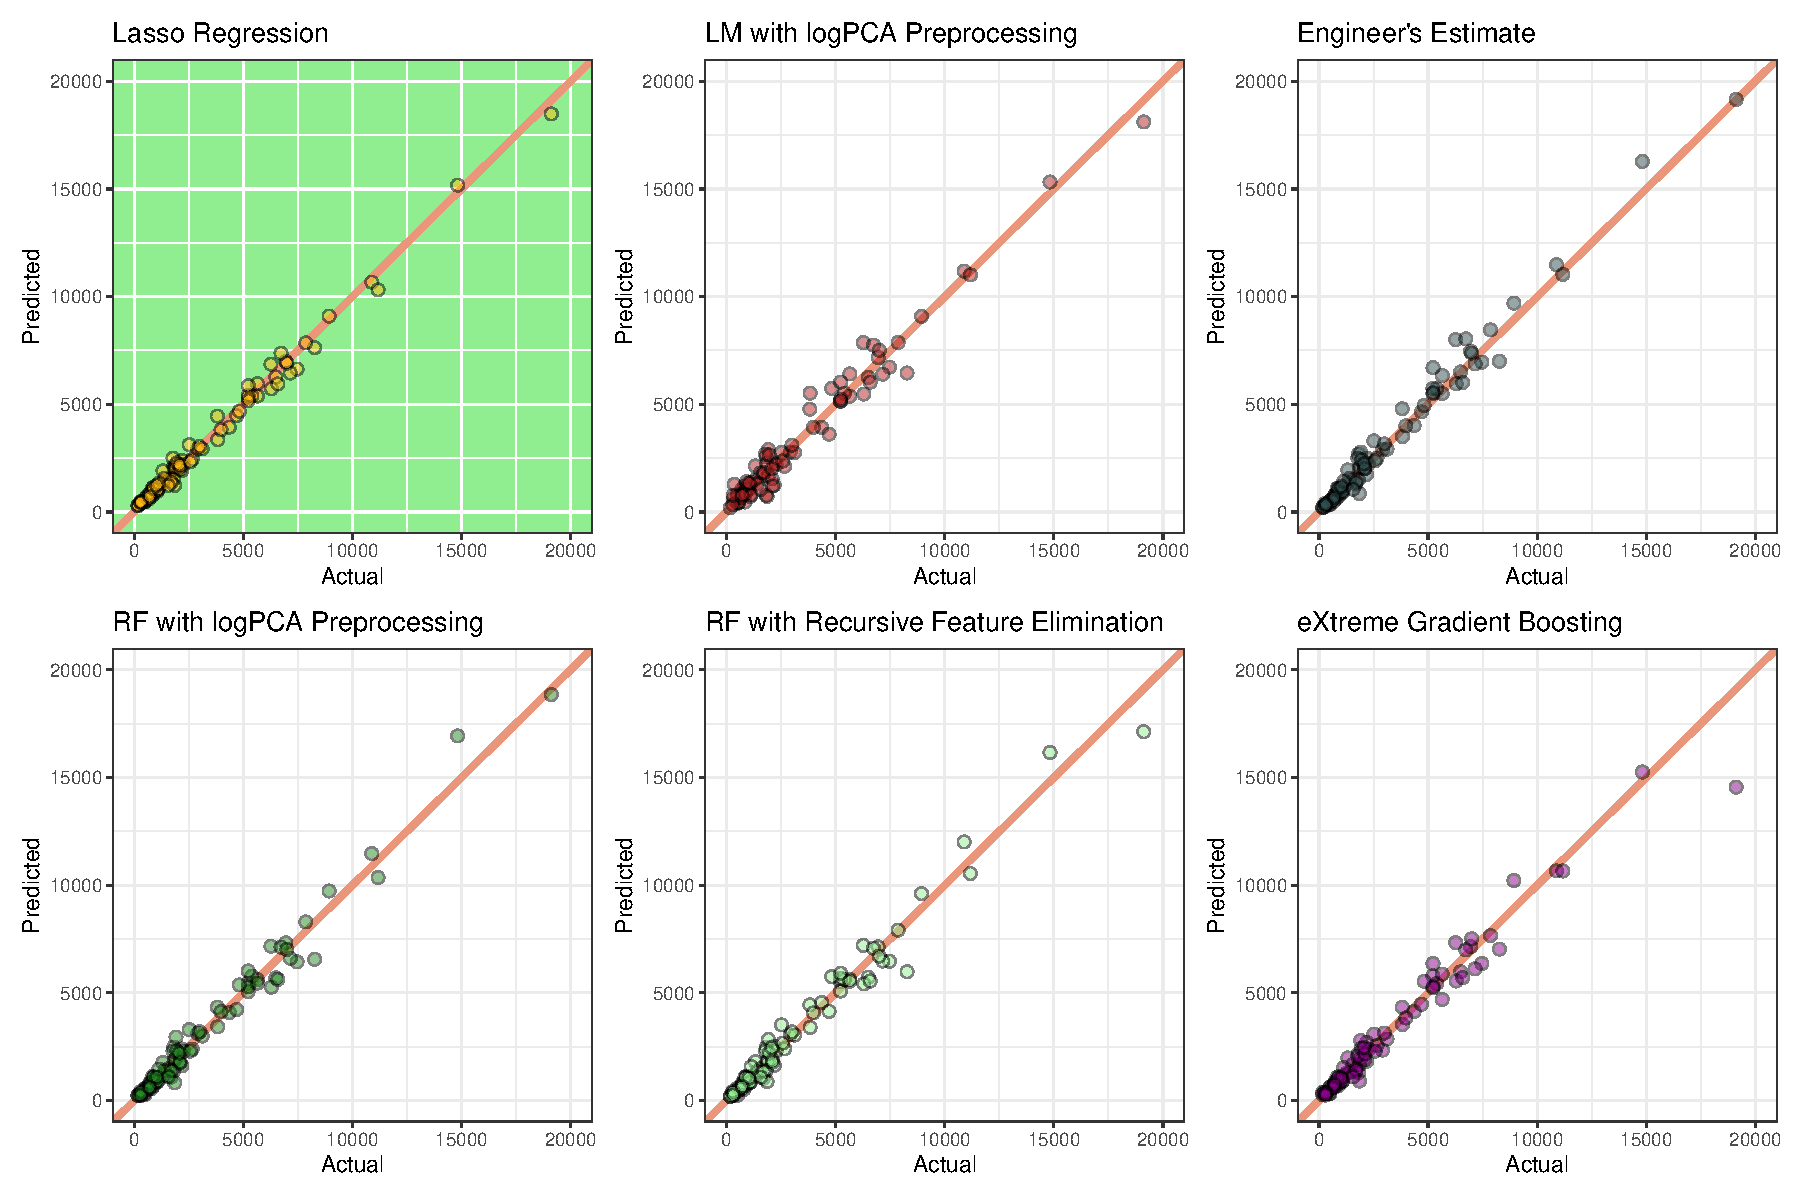
\includegraphics[width=0.9\linewidth]{./../figures/percomp_pres} 

}

\caption{Performance Comparison}\label{fig:unnamed-chunk-3}
\end{figure}
\end{frame}

\begin{frame}{Results: Out of Sample Performance}
\protect\hypertarget{results-out-of-sample-performance-1}{}
The following table lists the performance of the applied methods
utilizing linear and quadratic loss functions, i.e.,

\[ RMSE = \sqrt{\frac{1}{n}\sum_{i = 1}^n (\hat{y} - y)^2} ,\]
\[  MAE = \frac{1}{n}\sum_{i = 1}^n |\hat{y} - y|. \]

\begin{table}
\centering\begingroup\fontsize{7}{9}\selectfont

\begin{tabular}{l|r|r|r|r|r|r}
\hline
  & Lasso & Eng. Est. & logPCA\_RF & rfe\_RF & XGB & logPCA\_LM\\
\hline
RMSE & 326.1261 & 497.0567 & 509.7934 & 560.7600 & 671.6634 & 609.4673\\
\hline
MAE & 241.7894 & 327.9388 & 348.2869 & 373.1132 & 376.3191 & 448.2662\\
\hline
\end{tabular}
\endgroup{}
\end{table}
\end{frame}

\begin{frame}{Methods: Elastic Net}
\protect\hypertarget{methods-elastic-net}{}
Given the model matrix \(\mathbf{X} \in \mathbb{R}^{n\times p}\) and a
dependent variable \(\mathbf{y} \in \mathbb{R}^n\), we may formulate the
elastic net as a linear model that utilizes \(\ell_1\) and \(\ell_2\)
regularization. Further, suppose that \(\alpha \in [0, 1]\) and
\(t \in \mathbb{R}^+\), we can then define the elastic net estimator as
a constrained minimization problem,

\[ 
\boldsymbol{\hat{\beta}} = \underset{\boldsymbol{\beta}}{\text{arg min}} |\mathbf{y} - \mathbf{X}\boldsymbol{\beta}|^2,
\] subject to,

\[
(1 - \alpha)|\boldsymbol{\beta}|_1 + \alpha|\boldsymbol{\beta}|^2 \leq t. 
\] Where,

\[
|\boldsymbol{\beta}|_1 = \sum\limits_{i = 1}^{p}|\boldsymbol{\beta}_i|\text{ and } |\boldsymbol{\beta}|^2 = \sum\limits_{i = 1}^{p}\boldsymbol{\beta}_i^2.
\]
\end{frame}

\begin{frame}{Regularized Regression:
\href{https://www.desmos.com/calculator/59axr4plef}{Intuition}}
\protect\hypertarget{regularized-regression-intuition}{}
The best performing regularized model is a lasso regression model,i.e.,
\(\alpha = 0\). The lasso penalty shrinks some elements of the parameter
vector \(\hat\beta\) exactly to zero.

\begin{figure}

{\centering 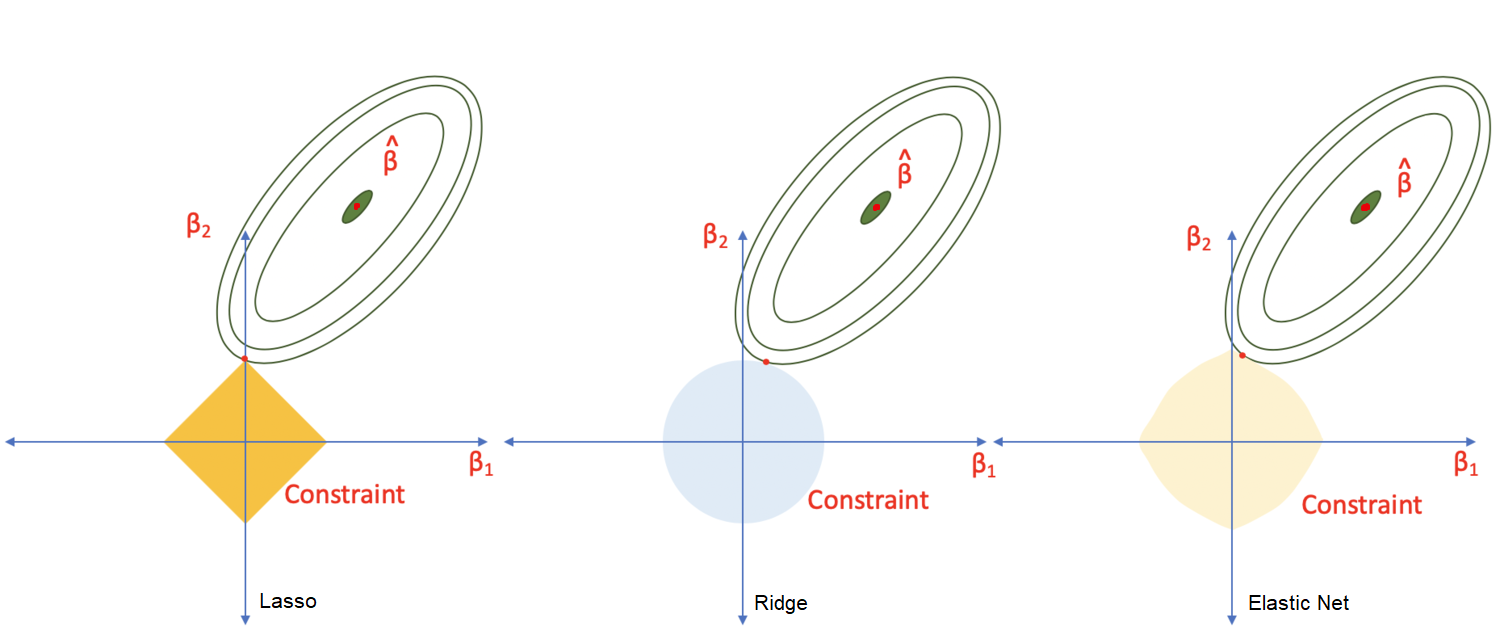
\includegraphics[width=0.9\linewidth]{./../figures/lasso_ridge} 

}

\caption{Regularization Utilizing Different Metrics (Toth 2022)}\label{fig:unnamed-chunk-5}
\end{figure}
\end{frame}

\begin{frame}{Why use Lasso Regression instead of OLS}
\protect\hypertarget{why-use-lasso-regression-instead-of-ols}{}
\begin{itemize}
\item
  Lasso allows us to fit a regression in cases where \(p>>n\).
\item
  Gauss Markov Theorem tells us that OLS is the best linear unbiased
  estimator but what if we do not mind a biased estimate?

  \begin{itemize}
  \tightlist
  \item
    Lasso offers a more flexible framework that allows us to optimize
    the bias variance tradeoff.
  \end{itemize}
\end{itemize}
\end{frame}

\begin{frame}{Bias Variance Tradeoff}
\protect\hypertarget{bias-variance-tradeoff}{}
\begin{figure}

{\centering 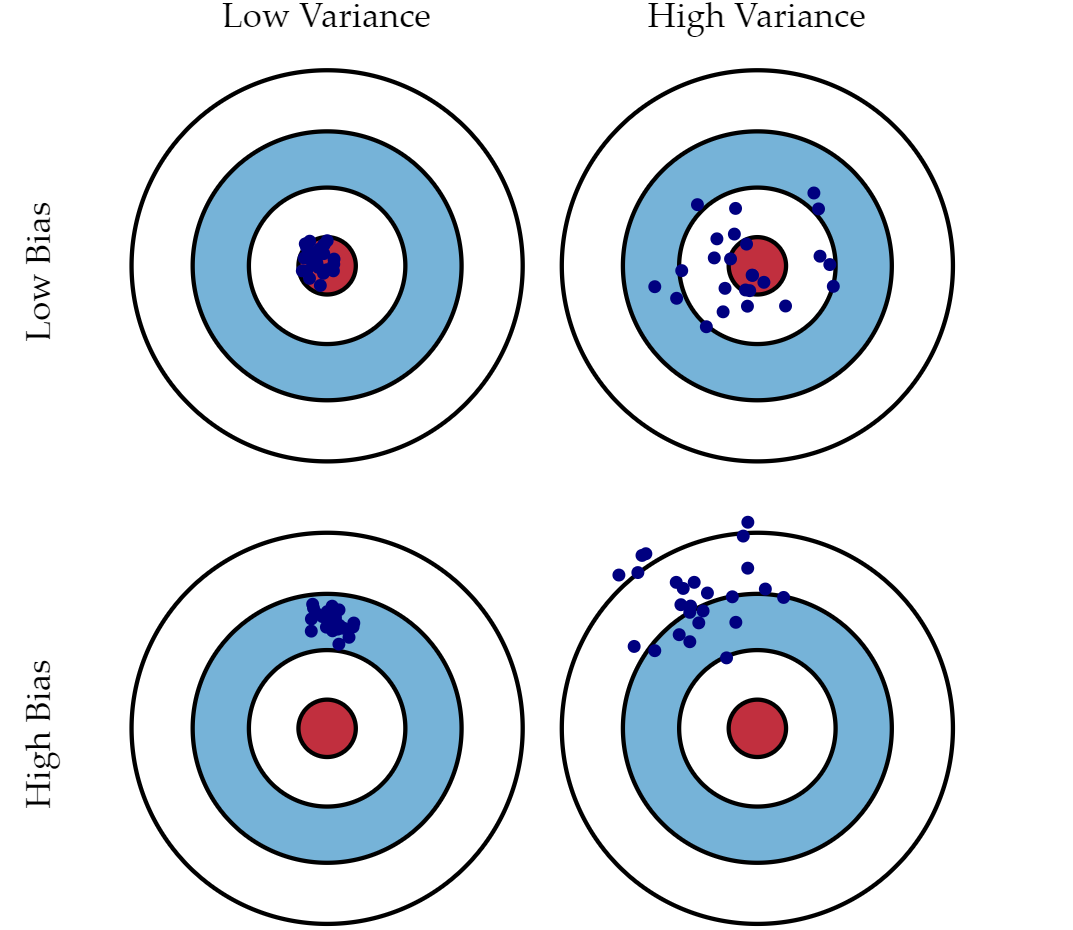
\includegraphics[width=0.7\linewidth]{./../figures/Bias_Variance} 

}

\caption{Bias Variance Tradeoff (Fortmann-Roe 2012)}\label{fig:unnamed-chunk-6}
\end{figure}
\end{frame}

\begin{frame}{Post Selection Inference: Motivation}
\protect\hypertarget{post-selection-inference-motivation}{}
The derivation of a test statistic for a single covariate in our model
usually assumes that the model is fixed, as if we knew ex ante which
variables we need to include.

\begin{itemize}
\tightlist
\item
  Why is it problematic if we use the Data to choose the variables in
  our model?

  \begin{itemize}
  \tightlist
  \item
    A pre-selection that minimizes some predictive error, will choose
    variables that have a relationship with the dependent variable
    \(\implies\) Type I error rate increases!
  \item
    Thus we need to correct our inferential procedure for this selection
    event!
  \end{itemize}
\item
  Very informally speaking, we could say, a predictor needs to suprise
  us twice. Once to make it into the model and then another time to
  reject the \(H_0\) of our significance test.
\end{itemize}
\end{frame}

\begin{frame}{Unsupervised Colusion Detection: Post-Selection Inference}
\protect\hypertarget{unsupervised-colusion-detection-post-selection-inference}{}
The R package that was used to obtain the test statistics to determine
the significance of our estimates is called \textit{selectiveInference}
by Tibshirani et al. (2019). It is based on a paper by the same authors
called
\textit{Post-selection inference for L1-penalized likelihood models}
(Taylor and Tibshirani 2016).

\begin{itemize}
\tightlist
\item
  The CV optimal value for our shrinkage parameter leads us to a model
  with 17/1085 variables.

  \begin{itemize}
  \tightlist
  \item
    11 of those are firm interaction terms.
  \item
    2 are description hit words.
  \item
    The remaining variables are Contract time, a county and a unique
    bidder identifier
  \end{itemize}
\item
  For the 430 auctions at hand no signficant interactions were detected!
\end{itemize}
\end{frame}

\begin{frame}{Links and Thesis Repository}
\protect\hypertarget{links-and-thesis-repository}{}
If you are interested to learn more about the application of machine
learning methods to predict procurement auction award prices you can
find my thesis including the data and the code here:
\textcolor{teal}{\textit{github.com/Base-R-Best-R/Auction}}.

If you are interested to learn more about post-selection inference.
Prof.~Loftus held a very insightful and easy to understand presentation
which is available on youtube:
\textcolor{teal}{\textit{youtube.com/watch?v=bQhEALoxoGE}}.

The link to the interactive Elastic-Net example may be found here:
\textcolor{teal}{\textit{desmos.com/calculator/skbksmodhd}}.
\end{frame}

\begin{frame}[allowframebreaks]{References}
\protect\hypertarget{references}{}
\hypertarget{refs}{}
\begin{CSLReferences}{1}{0}
\leavevmode\vadjust pre{\hypertarget{ref-tabulizer}{}}%
Leeper, Thomas J. 2018. \emph{Tabulizer: Bindings for Tabula PDF Table
Extractor Library}.

\leavevmode\vadjust pre{\hypertarget{ref-pdftools}{}}%
Ooms, Jeroen. 2022. \emph{Pdftools: Text Extraction, Rendering and
Converting of PDF Documents}.
\url{https://CRAN.R-project.org/package=pdftools}.

\leavevmode\vadjust pre{\hypertarget{ref-GarciaRodriguez2020}{}}%
Rodríguez, Manuel J. García, Vicente Rodríguez Montequín, Francisco
Ortega Fernández, and Joaquín M. Villanueva Balsera. 2020. {``Bidders
Recommender for Public Procurement Auctions Using Machine Learning: Data
Analysis, Algorithm, and Case Study with Tenders from Spain.''}
\emph{Complexity} 2020: 1--20.
\url{https://doi.org/10.1155/2020/8858258}.

\leavevmode\vadjust pre{\hypertarget{ref-tib2016}{}}%
Taylor, Jonathan, and Robert Tibshirani. 2016. {``Post-Selection
Inference for L1-Penalized Likelihood Models.''} arXiv.
\url{https://doi.org/10.48550/ARXIV.1602.07358}.

\leavevmode\vadjust pre{\hypertarget{ref-selectiveInference}{}}%
Tibshirani, Ryan, Rob Tibshirani, Jonathan Taylor, Joshua Loftus,
Stephen Reid, and Jelena Markovic. 2019. \emph{selectiveInference: Tools
for Post-Selection Inference}.
\url{https://CRAN.R-project.org/package=selectiveInference}.

\end{CSLReferences}
\end{frame}

\end{document}
